\documentclass[11pt]{article}
\usepackage[letterpaper,margin=1in]{geometry}
\usepackage[T1]{fontenc}
\usepackage{lmodern}
\usepackage{microtype}
\usepackage{amssymb}
\usepackage{needspace}
\usepackage{xcolor}
\usepackage{tabularx}
\usepackage{booktabs}
\usepackage{longtable}
\usepackage{array}
\usepackage{enumitem}
\usepackage{titlesec}
\usepackage{fancyhdr}
\usepackage{tikz}
\usetikzlibrary{arrows.meta,positioning,calc}
\usepackage[hidelinks]{hyperref}

\definecolor{accent}{HTML}{1F5F8B}
\definecolor{ph}{HTML}{B03A2E}
\definecolor{wf}{HTML}{555555}

\newcommand{\ph}[1]{\textcolor{ph}{[#1]}}
\newcolumntype{P}[1]{>{\raggedright\arraybackslash}p{#1}}
\newcolumntype{L}{>{\raggedright\arraybackslash}X}
\setlist{nosep,leftmargin=1.4em}
\titleformat{\section}{\large\bfseries\color{accent}}{\thesection.}{0.5em}{}
\titleformat{\subsection}{\normalsize\bfseries}{\thesubsection}{0.5em}{}
\titlespacing*{\section}{0pt}{14pt}{6pt}
\titlespacing*{\subsection}{0pt}{10pt}{4pt}
\renewcommand{\arraystretch}{1.25}

\pagestyle{fancy}
\fancyhf{}
\lhead{\small Project One Proposal: Movement Quest}
\rhead{\small \ph{Team Name}}
\cfoot{\small \thepage}

% ---------- wireframe phone macro ----------
% \phone{name}{x}{y}{screen number + title}{body tikz}
\newcommand{\phone}[5]{%
  \begin{scope}[shift={(#2,#3)}]
    \draw[rounded corners=6pt, thick] (0,0) rectangle (4,7);
    \draw[fill=gray!15] (0.15,6.25) rectangle (3.85,6.85);
    \node[font=\scriptsize\bfseries, anchor=west] at (0.25,6.55) {#4};
    \coordinate (#1) at (2,3.5);
    \begin{scope}[font=\tiny, color=wf]
      #5
    \end{scope}
  \end{scope}}
\newcommand{\wbox}[5]{\draw (#1,#2) rectangle (#3,#4); \node[font=\tiny, align=center] at ($({(#1+#3)/2},{(#2+#4)/2})$) {#5};}
\newcommand{\wbtn}[5]{\draw[fill=gray!30, rounded corners=2pt] (#1,#2) rectangle (#3,#4); \node[font=\tiny\bfseries] at ($({(#1+#3)/2},{(#2+#4)/2})$) {#5};}

\begin{document}

% ================= TITLE =================
\begin{center}
{\LARGE\bfseries\color{accent} Project One Proposal: Movement Quest}\\[4pt]
{\large Fitness Quest \& Training Challenges --- a playful, honest training logbook}\\[2pt]
{\small Topic category: Personal Momentum \quad$\cdot$\quad Flutter $\cdot$ SQLite $\cdot$ SharedPreferences $\cdot$ fully offline}
\end{center}

\begin{center}
\begin{tabularx}{0.92\textwidth}{@{}lL@{}}
\toprule
Course Section & \ph{e.g., CSC 4360 / Section 00X} \\
Team Name & \ph{Team Name} \\
Proposal Date & \ph{Date of submission} \\
Chosen Topic & Movement Quest (official topic brief, unchanged scope) \\
GitHub Repository URL & \ph{https://github.com/org/movement-quest} \quad (instructor added; all members are collaborators) \\
ClickUp Board URL & \ph{https://app.clickup.com/...} \quad (free plan; dated snapshot attached in Section~9) \\
Word Document File Name & \ph{TeamName\_Project1\_Proposal.docx} \\
Signed Statement & \ph{TeamName\_Signed\_Statement.pdf} (attached separately, Section~10) \\
\bottomrule
\end{tabularx}
\end{center}

% ================= 1 MEMBERS =================
\section{Proposed Group Members}

\begin{tabularx}{\textwidth}{@{}l l c L@{}}
\toprule
\textbf{Full Name} & \textbf{Student ID} & \textbf{Pathway} & \textbf{Expected Role / Responsibility} \\
\midrule
\ph{Member 1} & \ph{ID} & \ph{UG} & UI lead: Catalog/Dashboard and Create/Edit screens, navigation, reusable widgets \\
\ph{Member 2} & \ph{ID} & \ph{UG} & Data lead: SQLite schema, WorkoutPlan + TrainingLog CRUD, delete policy \\
\ph{Member 3} & \ph{ID} & \ph{UG} & Activity + testing lead: Detail/Activity flow, Settings, offline/restart tests \\
\ph{Member 4} & \ph{ID} & \ph{UG} & Helper + docs lead: Gear Match helper, AI\_FEATURE.md, report, demo script \\
\bottomrule
\end{tabularx}

\medskip
\needspace{12\baselineskip}
\noindent\textbf{Ownership map of implementation sections} (every section has a primary and a backup owner):

\begin{tabularx}{\textwidth}{@{}L l l@{}}
\toprule
\textbf{Implementation section} & \textbf{Primary} & \textbf{Backup} \\
\midrule
UI: five screen roles, reusable StatelessWidget/StatefulWidget components, forms, dialogs, accessibility & Member 1 & Member 3 \\
Data layer: SQLite helper, parameterized CRUD for both entities, cascade delete, SharedPreferences & Member 2 & Member 4 \\
Activity flow: start / log set / finish / reset, session grouping & Member 3 & Member 2 \\
Filter + aggregate: equipment filter, distinct-session count, total repetitions & Member 2 & Member 1 \\
Smart helper (Gear Match), baseline, evaluation cases, AI\_FEATURE.md & Member 4 & Member 3 \\
Testing: validation, offline restart on two devices/emulators, peer-driven revision & Member 3 & Member 1 \\
Documentation, report, slides, curated-question preparation & Member 4 & Member 2 \\
Demo video (20--25 min) segments & All (each presents own work) & --- \\
\bottomrule
\end{tabularx}

\smallskip
\noindent\textit{All members follow the undergraduate pathway. If any member is a graduate student, that member will additionally own the graduate extensions (advanced state management, architecture, background/local notification/file/animation, automated testing, and five held-out comparison cases).}

% ================= 2 SUMMARY =================
\section{Project Summary}

\subsection*{Problem and why it matters}
Students who do short workouts at home, in a dorm, or at the campus gym rarely keep an accurate record. They forget which routine they picked, lose count of sets, and a notes app cannot group sets into sessions or correct mistakes cleanly. \textbf{Movement Quest} turns a personal workout logbook into a quest menu: users build a small library of workout plans, run a workout by logging each set, and review and correct their honest history.

\subsection*{Target users}
College students and beginners who want a lightweight, private, offline log of self-chosen workouts, with no account and no data leaving the phone.

\subsection*{Scope boundaries (what the app is \emph{not})}
Movement Quest organizes \emph{user-entered} choices. It is not a trainer, injury assessor, or health recommender. It provides \textbf{no} medical advice, calorie predictions, injury-risk or safe-exertion predictions, wearable integration, camera form analysis, public rankings, or cloud records. Example routines in the seed data are illustrative, not prescriptive.

\subsection*{Core features}
\begin{itemize}
  \item Workout plan library with create/read/update/delete and an equipment filter.
  \item One complete workout flow: Start $\rightarrow$ log sets $\rightarrow$ Finish, or Reset (with confirmation).
  \item Correctable training history: view, edit, and delete individual set records.
  \item Accurate insights: completed-session count (distinct sessions, not set rows) and total repetitions.
  \item Persistent settings and one explainable, rule-based local smart helper (Gear Match).
\end{itemize}

\subsection*{Local-storage plan}
\begin{itemize}
  \item \textbf{SQLite} (\texttt{sqflite}): \texttt{workout\_plans} (parent) and \texttt{training\_logs} (child), foreign keys enabled, all queries parameterized.
  \item \textbf{SharedPreferences}: default effort, preferred equipment, dark mode, helper visibility.
  \item \textbf{No cloud storage of any kind.} ClickUp is used only for team coordination, never for app data.
\end{itemize}

\subsection*{Expected outcomes}
A tested Android APK that works fully offline on two devices/emulators, keeps records and settings across restarts, passes the ``sets are not sessions'' acceptance test, and includes a documented helper with a baseline and five evaluated cases.

\subsection*{Mapping to the equal-scope contract}
\begin{tabularx}{\textwidth}{@{}P{4.6cm}L@{}}
\toprule
\textbf{Required core item} & \textbf{How Movement Quest meets it} \\
\midrule
Five screen roles & Catalog/Dashboard, Create/Edit Plan, Detail/Activity, History/Insights, Settings (Section~4). No splash/login replaces a role. \\
Two related entities, CRUD for both & WorkoutPlan (parent) and TrainingLog (child) with full create/read/update/delete; confirmed cascade delete (Section~5). \\
Stateless + Stateful widgets & Stateless: \texttt{WorkoutCard}, \texttt{SetRow}, \texttt{StatTile}, \texttt{EmptyState}. Stateful: \texttt{ActivityScreen}, \texttt{PlanForm}, \texttt{SettingsScreen}. \\
Forms, lists/grids, buttons, dialogs & Validated plan form and set form; plan list and grouped history list; Save/Edit/Delete/Start/Finish/Reset buttons; confirmation dialogs. \\
Meaningful numeric control & Labeled \textbf{effort slider (1--5, Easy $\rightarrow$ Hard)} on the plan form and default-effort slider in Settings; numeric repetitions field with stepper buttons. \\
Activity workflow & Start $\rightarrow$ log sets $\rightarrow$ Finish / Reset with visible progress summary. \\
One filter & Equipment filter chips on the Catalog. \\
One aggregate & Distinct finished-session count and total repetitions on History/Insights and Dashboard. \\
Accessible gesture + button alternative & Swipe-to-delete on a set row, always paired with a visible Delete button. \\
Persistence across restart & SQLite records + SharedPreferences settings, verified by restart tests. \\
Offline on two devices & Tested on \ph{Pixel 7 emulator} and \ph{physical Android phone / second emulator}, airplane mode on. \\
Lifecycle cleanup and clear errors & Controllers disposed in \texttt{dispose()}; \texttt{mounted} checks after async writes; SnackBar errors with recovery guidance. \\
Peer-tested design revision & One wireframe/layout revision driven by peer feedback (Section~8.1). \\
Local smart helper + baseline & Gear Match (rule-based) vs.\ equipment-only baseline (Section~6). \\
\bottomrule
\end{tabularx}

% ================= 3 USER STORIES =================
\section{User Stories}
\begin{enumerate}
  \item \textbf{As a student with limited equipment,} I want to create workout plans tagged with the equipment they need \textbf{so that} I can quickly filter to a routine that fits what I have.
  \item \textbf{As someone working out,} I want to start a workout, log each set with its exercise and repetitions, and finish it \textbf{so that} I have an honest record of what I actually completed.
  \item \textbf{As a returning user,} I want to view, correct, and delete past sets and see how many sessions I have completed \textbf{so that} my history and progress stay accurate.
\end{enumerate}

% ================= 4 SCREENS =================
\section{Five Core Screens and Feature Pillars}

\begin{tabularx}{\textwidth}{@{}P{3.1cm}LL@{}}
\toprule
\textbf{Screen role} & \textbf{Purpose and key UI components} & \textbf{Flutter evidence / data used} \\
\midrule
1. Catalog / Dashboard & Main hub. Workout cards, equipment filter chips, completed-session count, Gear Match suggestion card, ``+ New Plan'' button. & Stateless \texttt{WorkoutCard}; reads all WorkoutPlans + distinct session count. \\
2. Create / Edit Plan & Validated title (required, 1--40 chars), equipment tag dropdown, plan note (exercise list), labeled effort slider 1--5. Save / Cancel; Delete (edit mode). & Stateful \texttt{PlanForm} with \texttt{Form}/\texttt{TextFormField} validators; insert/update WorkoutPlan. \\
3. Detail / Activity & Plan summary. \textbf{Start} $\rightarrow$ log set (exercise dropdown from bundled list + repetitions) $\rightarrow$ \textbf{Finish} or \textbf{Reset}. Live summary: ``3 sets $\cdot$ 36 reps''. & Stateful; generates a \texttt{sessionKey}; inserts TrainingLog rows; Finish marks the session finished. \\
4. History / Insights & Sets grouped by session. Edit repetitions or exercise label, delete a set (button + swipe). Totals: completed sessions, total reps. Empty state ``No sessions yet.'' & Full TrainingLog CRUD; aggregates recomputed after every edit/delete. \\
5. Settings & Default effort slider, preferred equipment, dark mode switch, show/hide helper toggle, ``About this helper'' explanation. & SharedPreferences; values restored on launch. \\
\bottomrule
\end{tabularx}

\medskip
\noindent\textbf{Six feature pillars (from the topic brief):}
\begin{enumerate}
  \item \textbf{Small editable plan library:} WorkoutPlan CRUD, equipment filtering, clear labels for user-created content. The exercise list is bundled choices in code, not a third entity.
  \item \textbf{Correctable set records:} create, read, edit, delete training logs; each row stores exercise label, repetitions, and session grouping so aggregates are explainable.
  \item \textbf{One complete workout flow:} Start, add progress, Finish, Reset. Finish never duplicates the last set or erases saved history. \textbf{Reset abandons only the current unfinished session} (its unfinished rows are removed); finished sessions are never touched.
  \item \textbf{Controls with visible units:} effort slider labeled 1--5, numeric repetitions (``reps''), Save/Edit/Delete buttons, reset confirmation; swipe gesture always has a button alternative.
  \item \textbf{Accurate personal summaries:} count distinct finished sessions, not set rows; recompute after edits/deletes; show empty history explicitly; never convert subjective effort into health claims.
  \item \textbf{Offline reliability:} persist records/settings, validate repetitions, guard repeated writes (Save/Finish disabled while a write is pending), show recovery guidance; test on two devices/emulators; peer-driven layout improvement.
\end{enumerate}

% ================= 5 DATA =================
\section{SQLite Data Model and Local Storage}

\begin{tabularx}{\textwidth}{@{}P{3.2cm}L P{4.2cm}@{}}
\toprule
\textbf{Entity} & \textbf{Fields (type)} & \textbf{CRUD surface} \\
\midrule
\textbf{WorkoutPlan} (parent) & id (INTEGER PK), title (TEXT, not null), equipmentTag (TEXT: None / Dumbbells / Resistance Band / Mat), planNote (TEXT), effortPreference (INTEGER 1--5) & Catalog + plan editor + detail deletion \\
\textbf{TrainingLog} (child) & id (INTEGER PK), workoutId (INTEGER FK $\rightarrow$ WorkoutPlan.id, ON DELETE CASCADE), sessionKey (TEXT), exerciseLabel (TEXT), repetitions (INTEGER $>$ 0), loggedAt (TEXT ISO-8601), sessionFinished (INTEGER 0/1) & Set form + history + log editor + deletion \\
\bottomrule
\end{tabularx}

\medskip
\begin{itemize}
  \item \textbf{SharedPreferences keys:} \texttt{default\_effort} (int 1--5), \texttt{preferred\_equipment} (string or none), \texttt{dark\_mode} (bool), \texttt{show\_helper} (bool).
  \item \textbf{Validation:} repetitions must be a positive integer (1--999); effort must be in the documented range 1--5; title required; non-numeric input shows an inline error.
  \item \textbf{Duplicate-write guard:} buttons are disabled while an insert/update is pending, so a double tap cannot create two rows.
  \item \textbf{Parent-delete policy: confirmed cascade.} Deleting a plan shows ``Delete \emph{Plan} and its \emph{N} logged sets? This cannot be undone.'' Only on confirmation are the plan and all its TrainingLog rows removed (\texttt{PRAGMA foreign\_keys = ON}).
  \item \textbf{Errors:} failed writes show a SnackBar with recovery guidance (``Could not save. Check storage and try again.'') and keep the user's input.
\end{itemize}

\subsection*{Must-solve challenge: sets are not sessions}
Every set logged during one workout shares one \texttt{sessionKey}. All session counts use \texttt{COUNT(DISTINCT sessionKey) WHERE sessionFinished = 1}, never the number of rows. Summaries are recomputed after every correction.

\noindent\textbf{Acceptance test:} log three sets in one finished session $\rightarrow$ count = 1. Delete one set $\rightarrow$ still 1. Delete the remaining two sets $\rightarrow$ 0. Delete a parent plan with logged sets $\rightarrow$ its sessions disappear from the count. Restart the app offline and confirm every value is unchanged.

% ================= 6 HELPER =================
\section{Required Local Smart Helper: Gear Match}

\begin{tabularx}{\textwidth}{@{}P{3.6cm}L@{}}
\toprule
Feature (from approved menu) & \textbf{Gear Match} --- organize a user-chosen routine. One suggestion card on the existing Catalog/Dashboard screen; no extra screen, entity, remote service, or large model. \\
User decision \& benefit & ``Which of my saved plans should I open next?'' The card surfaces a plan that fits the user's stated equipment and adds variety from the last session. \\
Success criterion & In our evaluation scenarios, the helper's top suggestion matches the reference choice in at least as many cases as the baseline, and every suggestion shows its reason. \\
Method label & \textbf{Rule-based scoring} (labeled honestly in the UI: ``Suggested by simple rules, not AI prediction''). \\
Inputs and units & (1) \texttt{preferred\_equipment} from SharedPreferences (category); (2) each plan's \texttt{equipmentTag} (category); (3) the \texttt{workoutId} of the most recent finished session, grouped by \texttt{sessionKey} (ID). Scores are unitless integer points. Effort and repetitions are deliberately \emph{not} inputs. \\
Method & +2 points if a plan's equipment matches the preference; +1 point if the plan differs from the most recent finished session. Sort by score descending, then by plan id ascending (stable tie rule). Equal session timestamps are resolved by the larger log id. Implemented as one pure Dart function. \\
Worked fixture & Preference = None (bodyweight). Plan A (None, not used last) = 3; Plan B (None, used last) = 2; Plan C (Dumbbells, not used last) = 1 $\Rightarrow$ suggest A. No exertion or repetitions are recommended. \\
Baseline & \textbf{Equipment match only, stable id ties} (the AI Lab baseline for this topic). Compared on the same valid inputs. \\
Explanation shown & ``Suggested: \emph{Plan A}. +2 matches your None preference, +1 different from your last session.'' \\
User override & Buttons \textbf{View plan} / \textbf{Not now}. The suggestion never starts a workout or changes intensity; the helper can be hidden in Settings. \\
No-data / invalid feedback & No plans $\rightarrow$ ``Add a plan first.'' No history $\rightarrow$ recent-use point omitted and the reason says so. No preference $\rightarrow$ match point omitted. Invalid data never reaches the helper because rows are validated before saving. \\
Owner & \ph{Member 4} (backup: \ph{Member 3}); documented in \texttt{AI\_FEATURE.md}. \\
\bottomrule
\end{tabularx}

\subsection*{Alternative considered}
The tiny nearest-neighbor recommender from the AI Lab walkthrough. We did not choose it initially because a new user has very few labeled examples, the distance between categorical tags is hard to explain, and the scoring rule produces a transparent reason that the user can check by hand. If the rule proves unhelpful in evaluation, we will document why and decide whether to revise.

\subsection*{Planned counterexample}
Preference = Dumbbells, but after a hard dumbbell session the user wants a light Mat stretching plan. Gear Match ranks the Mat plan low because it ignores what the user wants today. We will \textbf{preserve and disclose} this limitation (the reason text shows only equipment and variety) and rely on \emph{Not now} plus the full catalog, rather than inferring fatigue, which would be prohibited exertion advice.

\subsection*{Evaluation plan}
\begin{itemize}
  \item \textbf{Metric:} matches out of cases --- whether the top suggestion equals a reference choice written down \emph{before} running the helper. Both helper and baseline outputs are recorded for each valid case.
  \item \textbf{Sample:} the five required case types below plus \ph{5} additional valid fictional scenarios (sample size reported in AI\_FEATURE.md).
  \item No-data and invalid cases are judged on correct feedback, not on invented scores.
  \item For each case we record: case ID, inputs, expected behavior, actual behavior, pass/fail. We report one limitation and a justified revision or decision to retain the method.
\end{itemize}

\begin{tabularx}{\textwidth}{@{}P{1.6cm}P{2.3cm}LL c@{}}
\toprule
\textbf{ID} & \textbf{Case type} & \textbf{Inputs} & \textbf{Expected behavior} & \textbf{Pass/Fail} \\
\midrule
GM-1 & Normal & Pref = None; A(None, not last), B(None, last), C(Dumbbells, not last) & Scores 3/2/1; suggest A with full reason. Baseline: A and B tie at 2, id order $\rightarrow$ A. & TBD \\
GM-2 & Empty / insufficient & (a) No plans; (b) plans but no finished session & (a) ``Add a plan first.'' (b) Recent-use point omitted; reason says ``no history yet.'' & TBD \\
GM-3 & Invalid input & Set form: reps = 0, $-3$, or ``abc'' & Inline error, row not saved, no session created, helper output unchanged. & TBD \\
GM-4 & Boundary / tie & Two plans with equal score; and 3 set rows from one session for plan B & Lower id ranks first; the 3 rows count as one recent session (B gets 0 variety). & TBD \\
GM-5 & Counterexample & Pref = Dumbbells; user wants Mat stretch today & Mat plan ranked low; limitation disclosed; user picks via Not now / catalog. & TBD \\
\bottomrule
\end{tabularx}

\subsection*{Six critical-thinking decisions}
\begin{enumerate}
  \item \textbf{Define usefulness:} the decision is ``which saved plan next''; success is the match criterion above, not an ``AI'' badge.
  \item \textbf{Choose inputs:} equipment and last session only. Effort, repetitions, and any health data are excluded, because using them would imply ability or exertion judgments. Duplicated or edited set rows cannot inflate history because sessions are grouped by \texttt{sessionKey}.
  \item \textbf{Defend the method:} match (+2) outweighs variety (+1) because missing equipment makes a plan unusable, while repetition is only a mild preference. Tie rule: stable plan id.
  \item \textbf{Challenge the solution:} counterexample GM-5; limitation preserved and disclosed.
  \item \textbf{Compare fairly:} equipment-only baseline on the same inputs; if the baseline does as well, we will consider keeping the simpler method.
  \item \textbf{Preserve agency:} View plan / Not now, hideable helper, clear no-data messages. Equipment preference is useful but is \emph{not} a measure of ability; the card never claims readiness.
\end{enumerate}

% ================= 7 WIREFRAMES =================
\section{Proposed Wireframe (UI Visual Plan)}

\subsection{Screen map and navigation flow}
\begin{center}
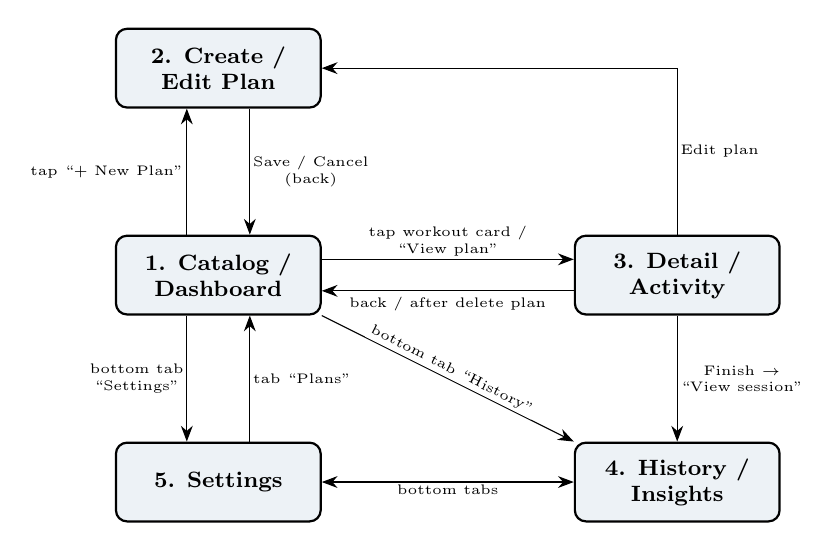
\begin{tikzpicture}[
  scr/.style={draw, rounded corners, thick, minimum width=2.6cm, minimum height=1cm, align=center, font=\footnotesize\bfseries, fill=accent!8},
  lab/.style={font=\tiny, align=center, fill=white, inner sep=1pt},
  >={Stealth[length=2mm]}]
  \node[scr] (cat) {1. Catalog /\\Dashboard};
  \node[scr, right=3.2cm of cat] (det) {3. Detail /\\Activity};
  \node[scr, above=1.6cm of cat] (edit) {2. Create /\\Edit Plan};
  \node[scr, below=1.6cm of det] (hist) {4. History /\\Insights};
  \node[scr, below=1.6cm of cat] (set) {5. Settings};
  \draw[->] ([xshift=-4mm]cat.north) -- node[lab, left]{tap ``+ New Plan''} ([xshift=-4mm]edit.south);
  \draw[->] ([xshift=4mm]edit.south) -- node[lab, right]{Save / Cancel\\(back)} ([xshift=4mm]cat.north);
  \draw[->] ([yshift=2mm]cat.east) -- node[lab, above]{tap workout card /\\``View plan''} ([yshift=2mm]det.west);
  \draw[->] ([yshift=-2mm]det.west) -- node[lab, below=1pt]{back / after delete plan} ([yshift=-2mm]cat.east);
  \draw[->] (det.north) |- node[lab, pos=0.25, right]{Edit plan} (edit.east);
  \draw[->] ([xshift=-4mm]cat.south) -- node[lab, left]{bottom tab\\``Settings''} ([xshift=-4mm]set.north);
  \draw[->] ([xshift=4mm]set.north) -- node[lab, right]{tab ``Plans''} ([xshift=4mm]cat.south);
  \draw[->] (det.south) -- node[lab, right]{Finish $\rightarrow$\\``View session''} (hist.north);
  \draw[->] (cat.south east) -- node[lab, sloped, above]{bottom tab ``History''} (hist.north west);
  \draw[<->] (set.east) -- node[lab, below]{bottom tabs} (hist.west);
\end{tikzpicture}
\end{center}
\noindent\textit{Navigation model:} a bottom navigation bar (Plans $\cdot$ History $\cdot$ Settings) links the three top-level screens; Create/Edit and Detail/Activity are pushed routes with a back action.

\subsection{Low-fidelity wireframes}
\begin{center}
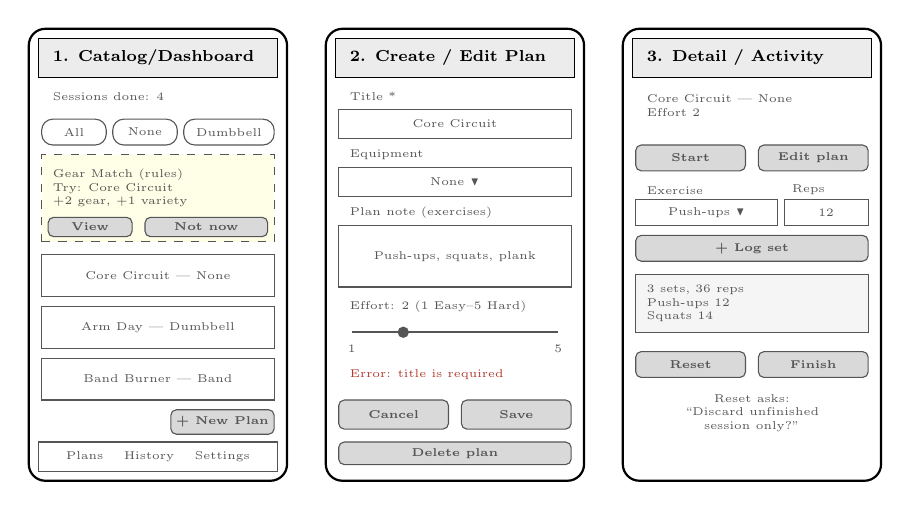
\begin{tikzpicture}[scale=0.82, every node/.style={transform shape}]
  % ---- Screen 1
  \phone{s1}{0}{0}{1. Catalog/Dashboard}{
    \node[anchor=west] at (0.25,5.95) {Sessions done: 4};
    \draw[rounded corners=4pt] (0.2,5.2) rectangle (1.2,5.6); \node at (0.7,5.4) {All};
    \draw[rounded corners=4pt] (1.3,5.2) rectangle (2.3,5.6); \node at (1.8,5.4) {None};
    \draw[rounded corners=4pt] (2.4,5.2) rectangle (3.8,5.6); \node at (3.1,5.4) {Dumbbell};
    \draw[dashed, fill=yellow!10] (0.2,3.7) rectangle (3.8,5.05);
    \node[align=left, anchor=north west] at (0.25,4.95) {Gear Match (rules)\\Try: Core Circuit\\+2 gear, +1 variety};
    \wbtn{0.3}{3.78}{1.6}{4.08}{View}
    \wbtn{1.8}{3.78}{3.7}{4.08}{Not now}
    \wbox{0.2}{2.85}{3.8}{3.5}{Core Circuit | None}
    \wbox{0.2}{2.05}{3.8}{2.7}{Arm Day | Dumbbell}
    \wbox{0.2}{1.25}{3.8}{1.9}{Band Burner | Band}
    \wbtn{2.2}{0.72}{3.8}{1.1}{+ New Plan}
    \draw (0.15,0.15) rectangle (3.85,0.6); \node at (2,0.38) {Plans \quad History \quad Settings};
  }
  % ---- Screen 2
  \phone{s2}{4.6}{0}{2. Create / Edit Plan}{
    \node[anchor=west] at (0.25,5.95) {Title *};
    \wbox{0.2}{5.3}{3.8}{5.75}{Core Circuit}
    \node[anchor=west] at (0.25,5.05) {Equipment};
    \wbox{0.2}{4.4}{3.8}{4.85}{None $\blacktriangledown$}
    \node[anchor=west] at (0.25,4.15) {Plan note (exercises)};
    \wbox{0.2}{3.0}{3.8}{3.95}{Push-ups, squats, plank}
    \node[anchor=west] at (0.25,2.7) {Effort: 2 (1 Easy--5 Hard)};
    \draw[thick] (0.4,2.3) -- (3.6,2.3); \fill (1.2,2.3) circle (2.5pt);
    \node at (0.4,2.05) {1}; \node at (3.6,2.05) {5};
    \node[color=ph, anchor=west] at (0.25,1.65) {Error: title is required};
    \wbtn{0.2}{0.8}{1.9}{1.25}{Cancel}
    \wbtn{2.1}{0.8}{3.8}{1.25}{Save}
    \wbtn{0.2}{0.25}{3.8}{0.6}{Delete plan}
  }
  % ---- Screen 3
  \phone{s3}{9.2}{0}{3. Detail / Activity}{
    \node[align=left, anchor=north west] at (0.25,6.1) {Core Circuit | None\\Effort 2};
    \wbtn{0.2}{4.8}{1.9}{5.2}{Start}
    \wbtn{2.1}{4.8}{3.8}{5.2}{Edit plan}
    \node[anchor=west] at (0.25,4.5) {Exercise};
    \wbox{0.2}{3.95}{2.4}{4.35}{Push-ups $\blacktriangledown$}
    \node[anchor=west] at (2.5,4.5) {Reps};
    \wbox{2.5}{3.95}{3.8}{4.35}{12}
    \wbtn{0.2}{3.4}{3.8}{3.8}{+ Log set}
    \draw[fill=gray!8] (0.2,2.3) rectangle (3.8,3.2);
    \node[align=left, anchor=north west] at (0.25,3.15) {3 sets, 36 reps\\Push-ups 12\\Squats 14};
    \wbtn{0.2}{1.6}{1.9}{2.0}{Reset}
    \wbtn{2.1}{1.6}{3.8}{2.0}{Finish}
    \node[align=center] at (2,1.05) {Reset asks:\\``Discard unfinished\\session only?''};
  }
\end{tikzpicture}
\end{center}

\begin{center}
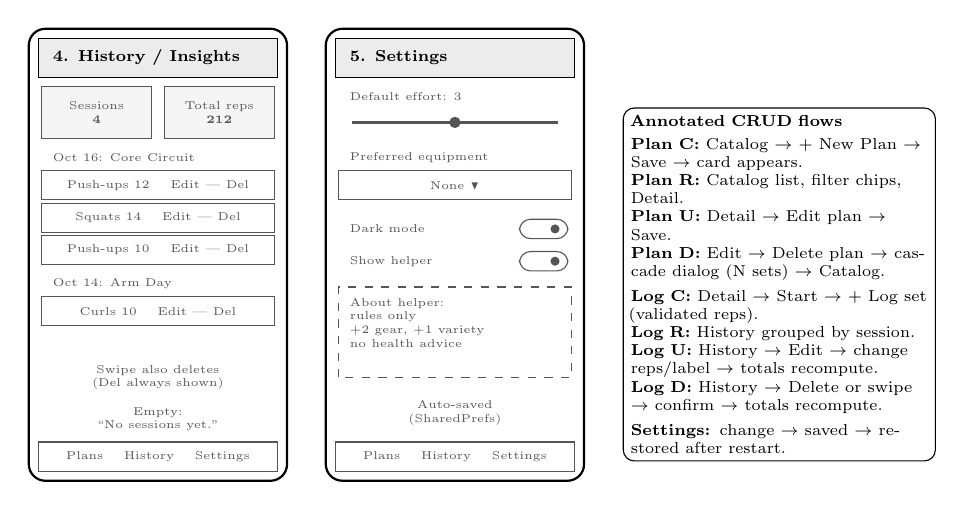
\begin{tikzpicture}[scale=0.82, every node/.style={transform shape}]
  % ---- Screen 4
  \phone{s4}{0}{0}{4. History / Insights}{
    \draw[fill=gray!8] (0.2,5.3) rectangle (1.9,6.1); \node[align=center] at (1.05,5.7) {Sessions\\\textbf{4}};
    \draw[fill=gray!8] (2.1,5.3) rectangle (3.8,6.1); \node[align=center] at (2.95,5.7) {Total reps\\\textbf{212}};
    \node[anchor=west] at (0.25,5.0) {Oct 16: Core Circuit};
    \wbox{0.2}{4.35}{3.8}{4.8}{Push-ups 12 \quad Edit | Del}
    \wbox{0.2}{3.85}{3.8}{4.3}{Squats 14 \quad Edit | Del}
    \wbox{0.2}{3.35}{3.8}{3.8}{Push-ups 10 \quad Edit | Del}
    \node[anchor=west] at (0.25,3.05) {Oct 14: Arm Day};
    \wbox{0.2}{2.4}{3.8}{2.85}{Curls 10 \quad Edit | Del}
    \node[align=center] at (2,1.6) {Swipe also deletes\\(Del always shown)};
    \node[align=center] at (2,0.95) {Empty:\\``No sessions yet.''};
    \draw (0.15,0.15) rectangle (3.85,0.6); \node at (2,0.38) {Plans \quad History \quad Settings};
  }
  % ---- Screen 5
  \phone{s5}{4.6}{0}{5. Settings}{
    \node[anchor=west] at (0.25,5.95) {Default effort: 3};
    \draw[thick] (0.4,5.55) -- (3.6,5.55); \fill (2.0,5.55) circle (2.5pt);
    \node[anchor=west] at (0.25,5.0) {Preferred equipment};
    \wbox{0.2}{4.35}{3.8}{4.8}{None $\blacktriangledown$}
    \node[anchor=west] at (0.25,3.9) {Dark mode}; \draw[rounded corners=4pt] (3.0,3.75) rectangle (3.75,4.05); \fill (3.55,3.9) circle (2pt);
    \node[anchor=west] at (0.25,3.4) {Show helper}; \draw[rounded corners=4pt] (3.0,3.25) rectangle (3.75,3.55); \fill (3.55,3.4) circle (2pt);
    \draw[dashed] (0.2,1.6) rectangle (3.8,3.0);
    \node[align=left, anchor=north west] at (0.25,2.95) {About helper:\\rules only\\+2 gear, +1 variety\\no health advice};
    \node[align=center] at (2,1.05) {Auto-saved\\(SharedPrefs)};
    \draw (0.15,0.15) rectangle (3.85,0.6); \node at (2,0.38) {Plans \quad History \quad Settings};
  }
  % ---- legend / CRUD flow
  \begin{scope}[shift={(9.2,0)}]
    \node[draw, rounded corners, align=left, text width=4.6cm, font=\scriptsize, anchor=south west] at (0,0.3) {%
      \textbf{Annotated CRUD flows}\\[2pt]
      \textbf{Plan C:} Catalog $\rightarrow$ + New Plan $\rightarrow$ Save $\rightarrow$ card appears.\\
      \textbf{Plan R:} Catalog list, filter chips, Detail.\\
      \textbf{Plan U:} Detail $\rightarrow$ Edit plan $\rightarrow$ Save.\\
      \textbf{Plan D:} Edit $\rightarrow$ Delete plan $\rightarrow$ cascade dialog (N sets) $\rightarrow$ Catalog.\\[3pt]
      \textbf{Log C:} Detail $\rightarrow$ Start $\rightarrow$ + Log set (validated reps).\\
      \textbf{Log R:} History grouped by session.\\
      \textbf{Log U:} History $\rightarrow$ Edit $\rightarrow$ change reps/label $\rightarrow$ totals recompute.\\
      \textbf{Log D:} History $\rightarrow$ Delete or swipe $\rightarrow$ confirm $\rightarrow$ totals recompute.\\[3pt]
      \textbf{Settings:} change $\rightarrow$ saved $\rightarrow$ restored after restart.};
  \end{scope}
\end{tikzpicture}
\end{center}

\subsection{Key use cases and transitions}
\begin{enumerate}
  \item \textbf{Plan a workout:} Catalog $\rightarrow$ tap ``+ New Plan'' $\rightarrow$ fill form $\rightarrow$ Save $\rightarrow$ back to Catalog with the new card.
  \item \textbf{Do a workout:} Catalog $\rightarrow$ tap card (or Gear Match ``View'') $\rightarrow$ Detail $\rightarrow$ Start $\rightarrow$ Log set (repeat) $\rightarrow$ Finish $\rightarrow$ session saved, count updates.
  \item \textbf{Correct history:} bottom tab History $\rightarrow$ Edit or Delete a set $\rightarrow$ totals recompute immediately.
  \item \textbf{Personalize:} bottom tab Settings $\rightarrow$ change preference $\rightarrow$ Catalog suggestion reflects it.
\end{enumerate}

\subsection{Edge cases shown in the wireframes}
\begin{itemize}
  \item \textbf{Empty state:} no plans $\rightarrow$ Catalog shows ``Add a plan first''; no sets $\rightarrow$ History shows ``No sessions yet.''
  \item \textbf{Validation error:} empty title or reps $\le 0$ / non-numeric $\rightarrow$ inline red error; Save disabled.
  \item \textbf{Failed save:} SnackBar ``Could not save. Try again.'' and form input kept.
  \item \textbf{Missing data:} no preference or no history $\rightarrow$ helper omits that point and says so.
\end{itemize}

% ================= 8 TESTING / ITERATION =================
\section{Test Cases and Iterative Design}

\begin{tabularx}{\textwidth}{@{}P{0.9cm}LLL@{}}
\toprule
\textbf{ID} & \textbf{What is tested} & \textbf{Expected result} & \textbf{Revision action if it fails} \\
\midrule
T1 & Create plan with empty title & Inline error, nothing saved & Fix validator / error text \\
T2 & Log reps = 0, $-1$, ``abc'' & Rejected with message & Tighten numeric parsing \\
T3 & Double-tap Save / Finish & Exactly one row / one finished session & Add pending-write guard \\
T4 & Sets-vs-sessions acceptance test (Section~5) & 1 $\rightarrow$ 1 $\rightarrow$ 0, unchanged after restart & Fix grouping query \\
T5 & Delete plan with logged sets & Dialog shows N; plan + sets removed; counts update & Fix cascade / refresh \\
T6 & Reset during active session & Only unfinished rows removed; history intact & Scope reset query by sessionKey \\
T7 & Change settings, force-close, reopen & Settings and records restored & Fix SharedPreferences load order \\
T8 & Airplane mode on two devices/emulators & All features work offline & Remove any network dependency \\
T9 & Large text scaling and screen-reader labels & No overflow; controls labeled & Adjust layout / semantics \\
T10 & Gear Match cases GM-1 to GM-5 & As in Section~6 & Revise or disclose limitation \\
\bottomrule
\end{tabularx}

\subsection{Peer review and iteration plan}
\begin{enumerate}
  \item After the UI/navigation checkpoint (Oct 21), two peers outside the team complete three tasks on the wireframe/prototype: create a plan, log and finish a 3-set workout, correct one set.
  \item We collect: task success, time to complete, where they hesitated, and one ``what confused you'' answer per screen.
  \item We revise at least one layout based on that feedback (for example, moving Finish away from Reset to prevent mis-taps), record the before/after screenshots and the reason, and retest the same task.
\end{enumerate}

% ================= 9 CLICKUP =================
\section{Project Management: ClickUp and GitHub}

\begin{itemize}
  \item \textbf{Board URL:} \ph{https://app.clickup.com/...} (free plan; used only for coordination, never app storage).
  \item \textbf{Kanban workflow:} Backlog $\rightarrow$ To Do $\rightarrow$ In Progress $\rightarrow$ Review (PR open) $\rightarrow$ Done.
  \item \textbf{WIP limits:} In Progress = 2 cards per person (8 team-wide); Review = 4. A card moves to Done only when its acceptance criteria pass and its PR is merged.
  \item \textbf{Every card has:} an owner, acceptance criteria, a due date, and (when done) a link to the commit/PR and test evidence.
  \item \textbf{Dated snapshots:} October 18 (planning snapshot, attached below), 21, 24, and 28.
  \item \textbf{GitHub:} \ph{repo URL}; one feature branch per card, pull requests reviewed by another member, at least 20 meaningful commits per person.
\end{itemize}

\begin{tabularx}{\textwidth}{@{}P{3.1cm}L P{2.1cm}P{1.8cm}@{}}
\toprule
\textbf{Milestone} & \textbf{Tasks and acceptance criteria} & \textbf{Owner} & \textbf{Due} \\
\midrule
Proposal & Proposal, wireframes, signed statement, board snapshot uploaded & All & Oct 18 \\
UI / navigation & Five screens navigable with bottom bar; plan form validates; peer review done & M1, M3 & Oct 21 \\
Core functionality & Vertical slice, then full CRUD for both entities; cascade delete; workout flow; settings persist; sets-vs-sessions test passes & M2, M3 & Oct 24 \\
Helper & Gear Match + baseline on Catalog; GM-1 to GM-5 recorded & M4 & Oct 25 \\
Verify \& improve & Offline/restart on two devices; peer-driven revision; bug fixes & M3, M1 & Oct 26 \\
Final submission & APK, report, AI\_FEATURE.md, slides, curated questions, 20--25 min video & All & Oct 28 \\
\bottomrule
\end{tabularx}

\medskip
\noindent\ph{Insert readable, dated October 18 ClickUp board snapshot here.}
% \includegraphics[width=\textwidth]{clickup_oct18.png}

% ================= 10 SIGNED =================
\section{Signed Statement Attachment}
The completed team acknowledgment, with all names, signatures, and dates readable, is attached separately as \ph{TeamName\_Signed\_Statement.pdf} (or a clear PNG/JPG scan), including any continuation sheet. Development will begin only after instructor-team approval of this proposal.

\end{document}
